\documentclass[border=1cm,tikz]{standalone}

\usetikzlibrary{arrows.meta}
\usetikzlibrary{decorations.pathmorphing}

\definecolor{lightblue}{rgb}{0.149,0.545,0.824}
\definecolor{darkred}{rgb}{0.647,0.129,0.149}
\definecolor{green}{rgb}{0.365, 0.592, 0.157}

\begin{document}

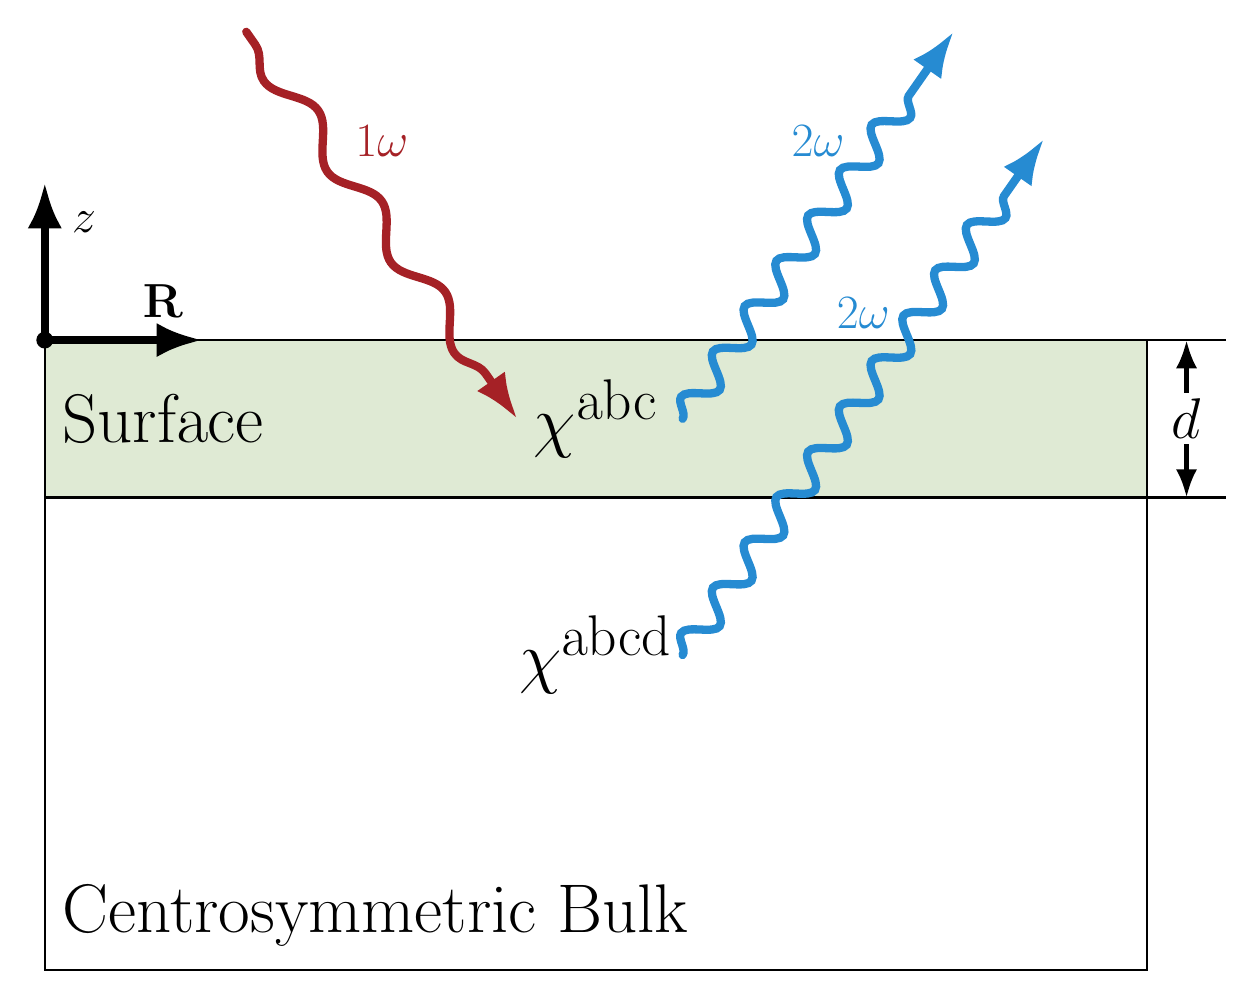
\begin{tikzpicture}

% membrane cell
\filldraw [thick,fill=green,fill opacity=0.2] (0,6) rectangle (14,8);
\draw [thick] (0,0) rectangle (14,8);

% d distance indicator
\draw [thick] (15,6) -- (14,6) -- (14,8) -- (15,8);
\draw [Latex-Latex,ultra thick] (14.5,6) -- (14.5,8);
\node at (14.5,7.0) [fill=white,inner sep=2pt] {\huge $d$};

% axes
\draw [Latex-Latex,line width=3pt] (2,8) -- (0,8) -- (0,10);
\filldraw [color=black] (0,8) circle (0.1);
\node at (0.5,9.5) {\LARGE $z$};
\node at (1.5,8.5) {\LARGE $\mathbf{R}$};

% light beams yo
\draw [Latex-,decorate,decoration={snake,amplitude=5,segment length=40,pre length=20},line width=3pt,darkred,line cap = round] (6,7) -- ++(125:6) node [draw=none,midway,above=20] {{\LARGE $1\omega$}};
\draw [-Latex,decorate,decoration={snake,amplitude=5,segment length=20,post length=20},line width=3pt,lightblue,line cap = round] (8.1,7) -- ++(55:6) node [draw=none,midway,above=20] {{\LARGE $2\omega$}};
\draw [-Latex,decorate,decoration={snake,amplitude=5,segment length=20, post length=20},line width=3pt,lightblue,line cap = round] (8.1,4) -- ++(55:8) node [draw=none,midway,above=20] {{\LARGE $2\omega$}};

% some text
\node at (7,7) {\Huge $\chi^{\mathrm{abc}}$};
\node at (7,4) {\Huge $\chi^{\mathrm{abcd}}$};
\node at (1.5,7) {\Huge Surface};
\node at (4.2,0.7) {\Huge Centrosymmetric Bulk};

\end{tikzpicture}

\end{document}
